%Pick your document class 
\documentclass{report}
%Insert necessary packages 
%This package will change the margins to .5in. If you want something different then change it
\usepackage[margin=0.5in]{geometry}
%This package is for citing your sources 
\usepackage[backend=biber]{biblatex} 
%This package will allow you to jump to your sources 
\usepackage{hyperref} 
%This package is used for writing math equations 
\usepackage{amsmath}
%This package will be used for inserting our charts and graphs 
\usepackage{graphicx}
%This line points to the location of the file where you cite your sources 
\addbibresource{my.bib}

%Begin document
\begin{document} 
%Choose formatting 

\hfill Submitted by: Christian Foster 

\hfill Lab partners: Pat, Mike, and Jules 

\hfill Data Collected: 28 February 2017 

\hfill Report Submitted: 25 April 2017

%Format for title of paper 
\begin{center}
\fontsize{18pt}{12pt}\selectfont 
\LaTeX (Lab Report Tutorial) A descriptive title that says exactly what you did and what you found
\end{center}
%Start Abstract Section 
\textbf{Abstract:} Short version of concluding paragraph, include major discoveries, keep it short and state method.
%Introduction Section, flushleft will start the paragraph on the next line
\begin{flushleft}
\textbf{Introduction:} This section is background. It explores the ideas behind your experiment. Start with a topic sentence that states the purpose of the lab. Define any terms in this section The format is up to your teacher and citations must footnote citations. In \LaTeX this is very easy. It just takes a bit of learning. In this example we will be using biblatex with biber. First you must find a source for citation. In our case we will use Mr.Madara's example lab report. He cites a source that says ``Tacos require meat and cheese at all times''. To do this we will make a .bibfile. Now a source was made in my.bib called taco. To cite this source as a footnote use supercite. This example can be found on Mr.Madara's website:\supercite{madara}
\end{flushleft}
%So we need to cite a source for tacos requiring meat at all times. You have to cite it using the name of the citation in your .bib file. In this case I named the citation taco, so I will use taco
\hspace{6ex}There is a skill needed to make tacos. ``Tacos require meat and cheese at all times''\supercite{taco}. 
The amount of meat and cheese must follow the equation\supercite{taco}
%This is where writing citations in latex comes into play. If you didn't write \usepackage{amsmath} at the top then your file won't compile.
\begin{equation}\label{meateq}
\text{Meat} = \text{cheese} \times d^2
\end{equation}
where $d$ represents the diameter of the taco. The amount of sauce added  follows the equation\supercite{taco}
\begin{equation}\label{sauce}
\text{Sauce} = \text{(cheese + meat) / 2}
\end{equation}
%These equations can be later referenced using \eqref{meateq} and \eqref{sauce}
The process of making tacos is called tacofication\supercite{taco}. The chef must first master this process before trying more creative versions. 
\begin{flushleft}
\textbf{Experimental:}
\end{flushleft}
\begin{itemize}
\item{Materials go here in a bulleted list}
\item{The materials are not listed in more proffesional papers}
\item{A teacher may or may not require you to list them}
\end{itemize}
\hspace{6ex}The procedure of the lab goes here. It MUST be in past tense because you already performed the lab. NO pieces of data. NO people words or lab partner names. The program that you use for graphing must be cited in the last sentence like All data was entered into Libreoffice Calc\supercite{libreoffice}.
\begin{flushleft}
\textbf{Results/Conclusions:}This section is start with a general discussion of what you saw with your eyes. Your first paragraph will have qualitative data. This section will also contain embedded data tables. This is a litle difficult with latex. You will neeed to take screenshots of your graphs and charts using some screenshot program. If you are on windows you can use the snipping tool. If you are using linux like a good little boy then you can set binds with scrot or use shutter. You could try to create latex tables but I find this easier.
\end{flushleft}
%In latex you will use \includegraphics{nameofgraphic} to insert an image 
\begin{center}
%If the table looks ugly you can scale it
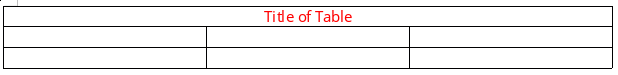
\includegraphics[scale=.7]{examplechart}
\end{center}
\begin{flushleft} 
\hspace{6ex}After the table you should describe what is in it by saying things such as ``the first column shows'' If you need to say you did some math you should reference an equation from the introduction using eqref. Ex.= ``The amount of sauce was found using equation\eqref{sauce}. This prevents you from writing the equation over and over. You should include your graphs after you have included all of your tables. 
\end{flushleft}
\begin{flushleft}
Graph 1: 
\end{flushleft}
\begin{center}
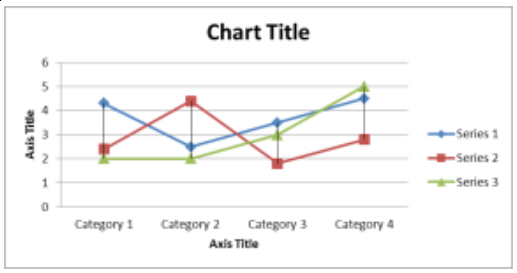
\includegraphics[scale=.7]{graph}
\end{center}
\begin{flushleft}
You need labels on x-axis, y-axis, and title. You should comment on any patterns you see in the graph such as plateaus or spikes in slope.
\end{flushleft}
\hspace{6ex}This paragraph should be about your percent error. You should include a percent error for all major discoveries. If your percent error is 5\% or less you can claim to be accurate. You need to give possible sources of error that are not your fault or something you could fix. Think of it as being employed because you would not want to give an excuse for bad data that would get you fired. There are plenty of sources of error that you have no control over. You should also make sure the source of error matches your data. If your result was too high you would not want to give a source of error that explains low answers.  You should conclude this section with a next logical step that you would take in the experiment.
\begin{flushleft}
\hspace{6ex}This should be your concluding paragraph. It should start with the purpose of the lab. You should give your major discoveries and method used. You should say if you were accurate. You can then give any final thoughts.
\end{flushleft}
%To load up your citations you must run biber. Once you compile your latex file, you run biber on your file then recompile your latex file and you are all set. You won't have to run biber everytime you compile your latex file, you only have to run it when you change or add a citation. 
\printbibliography
\begin{flushleft}
\hspace{6ex}As you can see \LaTeX  makes citations a breeze. It is very different from word or google docs so it does take some learning but once you start writing with it you realize how great it is.
\end{flushleft}
%To start your calculations on another page you must use \newpage
\newpage 
\begin{flushleft}
This page can be done by hand if you use blue or black ink and write on blank computer paper. You should include one example of every type of calculation. All numbers need units. Each calculation should have three parts: the equation to be used without any data plugged in, the equation with your data plugged in, and the answer.
\end{flushleft}
\begin{flushleft}
\hspace{6ex}Equations in \LaTeX are usually written with a \$ in front. The examples that Madara uses in his template is really simple so it can be written normally.
\end{flushleft}
\begin{flushleft}
Density = Mass/Volume \hfill

Density = 5 grams/0.5mL \hfill

Density = 10 grams/mL \hfill

\end{flushleft}
\begin{flushleft}
Just to give you some idea of what more complex equations look like in \LaTeX, here is an example formula for freezing point depression.
\end{flushleft}
\begin{flushleft} 
$\Delta T_{f}=(K_{f})(m)$ 
\end{flushleft}
\begin{flushleft} 
Now see, it isn't that bad. Now you can go ahead and write your lab report in \LaTeX using this as a guide.
\end{flushleft}
\end{document}
